\documentclass[11pt,a4paper]{article}

\usepackage[utf8]{inputenc}
\usepackage[T1]{fontenc}
\usepackage{lmodern}
\usepackage[english]{babel}

\usepackage[a4paper,margin=1in]{geometry}
\usepackage{setspace}
\usepackage{graphicx}
\usepackage{booktabs}
\usepackage{amsmath, amssymb}
\usepackage{hyperref}
\usepackage{enumitem}
\usepackage{float}
\usepackage{multirow}
\usepackage{array}
\usepackage{xcolor}

\hypersetup{
    colorlinks=true,
    linkcolor=blue,
    urlcolor=blue,
    citecolor=blue
}

\title{Comparison of AdamW, Muon and Hybrid Optimization for Full Fine-Tuning of Qwen2.5-0.5B}
\date{2026}
\author{Ilya Saenko\\
    \texttt{sia3301@yandex.ru}}

\begin{document}

\maketitle

\begin{abstract}
	Optimizers based on orthogonal gradient updates, such as Muon, have recently
	emerged as promising alternatives to AdamW for training large-scale language
	models. However, their behavior under resource-constrained conditions small
	model sizes, limited batch sizes, and short training budgets remains
	underexplored. In this work, we conduct a systematic empirical comparison of
	three optimization strategies for continued pre-training of the Qwen2.5-0.5B
	language model: (1) a standard AdamW baseline, (2) a Moonlight Muon
	configuration that applies orthogonal gradient updates to internal 2D weight
	matrices while using AdamW for remaining parameters, and (3) a depth-stratified
	Hybrid approach that restricts Muon to the first 12 transformer layers and
	delegates deeper layers and scalar parameters to AdamW. All methods are
	evaluated over 1500 training steps on the OpenWebText corpus and assessed
	zero-shot on five reasoning benchmarks: ARC-Challenge, ARC-Easy, HellaSwag,
	PIQA, and Winogrande. Our results show that all three optimizers converge at
	nearly identical rates and achieve comparable downstream accuracy, with the
	Hybrid approach reaching the highest aggregate score of 0.5260. Despite the
	overall parity in performance, neither Muon nor the Hybrid method introduces
	training instability, confirming their safe applicability as drop-in replacements
	for AdamW even under small-batch, small-model regimes. We discuss the
	contributing factors to this parity namely gradient noise at small batch sizes
	and the well-conditioned optimization landscape of a compact model.
\end{abstract}

\section{Introduction}

Optimizer choice critically impacts language model training outcomes.
While AdamW has become the standard for transformer models, Muon-which
applies orthogonalization to gradient matrices-has shown promise at scale.
However, Muon's effectiveness in resource-constrained environments remains
understudied.

This report compares three optimization strategies for continued pre-training
of Qwen2.5-0.5B: standard AdamW, Moonlight Muon (applying Muon to 2D matrices
and AdamW to other parameters), and a novel Hybrid approach (using Muon only
in the first 12 transformer layers). Our controlled experiments maintain
identical training conditions across all configurations.

Results show all three optimizers achieve comparable convergence rates and
benchmark performance (within 0.3 percentage points). The Hybrid approach
marginally outperforms both alternatives (0.5260 vs. 0.5254 for AdamW and 0.5230
for Muon). Our findings suggest that while Muon and Hybrid approaches are
viable AdamW alternatives in resource-constrained settings, the orthogonalization
benefits may be more pronounced with larger batch sizes where gradient noise
is reduced.


\section{Experiments}

\subsection{Experimental Setup}
For all experiments, we use a single NVIDIA RTX 4090 GPU with 24\,GB of VRAM
and a system with 62\,GB of RAM. To ensure reproducibility, we fix the random
seed to 42 across all stochastic operations in Python, NumPy, and PyTorch.
In addition, we enable deterministic algorithms in PyTorch and configure cuDNN
for deterministic execution, at the cost of potentially reduced performance.

We choose Qwen2.5-0.5B as the base model for all experiments due to its moderate
size, which allows for reasonable training times while remaining representative
of modern language model architectures. The model is loaded in bfloat16
precision to improve memory efficiency and computational performance. We also
enable gradient checkpointing to mitigate memory constraints and use scaled
dot-product attention (SDPA) for transformer computations.

\subsection{Training Configuration}
All models are trained for 1500 steps with an effective batch size of 64
(a per-device batch size of 8 with 8 gradient accumulation steps).
Each micro-batch loss is normalized by the number of gradient accumulation
steps before the backward pass, so that the effective gradient magnitude
remains consistent with a single-step batch of size 64.
The maximum sequence length is fixed at 1024 tokens in all experiments.
We use a cosine learning rate schedule with a warmup of 50 steps.

Training is performed with \texttt{bfloat16} automatic mixed precision
(\texttt{torch.amp.autocast}) enabled. Since bfloat16 does not require
loss scaling, the gradient scaler is disabled throughout all experiments.

No gradient clipping is applied (\texttt{max\_grad\_norm = None}),
allowing us to observe the unmodified gradient dynamics of each optimizer
and ensure a fair comparison.

For training data, we use the \texttt{Elriggs/openwebtext-100k} dataset,
which provides a balanced and diverse corpus of web text.


\subsection{Optimizers}

To facilitate the use of multiple optimization strategies simultaneously,
we implemented a straightforward \texttt{HybridOptimizer} wrapper class. It
inherits from \texttt{torch.optim.Optimizer} and accepts a list of instantiated
standard optimizers. Its primary function is to verify that the optimizers
operate on strictly disjoint parameter sets, preventing parameter overlap,
while synchronizing their \texttt{step} and \texttt{zero\_grad} operations.
Using this utility, we compare three optimization approaches:

\begin{enumerate}
	\item \textbf{AdamW Baseline.}
	      We use the standard PyTorch AdamW optimizer applied to all model
	      parameters. The hyperparameters are set to a learning
	      rate of $5 \times 10^{-5}$, $\beta = (0.9, 0.999)$, $\epsilon = 10^{-8}$,
	      and weight decay of $10^{-2}$. This serves as our baseline,
	      representing the de facto standard for training
	      transformer-based language models.

	\item \textbf{Moonlight Muon.}
	      This approach utilizes the standard Muon optimizer from the
	      \texttt{torch.optim} library in combination with AdamW
	      via our \texttt{HybridOptimizer} wrapper. The model
	      parameters are divided into two distinct groups. Muon
	      is assigned exclusively to internal 2D weight matrices
	      (excluding embeddings and language model heads). AdamW handles all
	      remaining parameters, including 1D tensors, biases, LayerNorm weights,
	      embeddings, and heads.

	      For the Muon optimizer, we use a learning rate of $2 \times 10^{-4}$,
	      momentum of $0.95$ with Nesterov acceleration enabled, weight
	      decay of $0.01$, $\epsilon = 10^{-8}$, and $5$ Newton-Schulz
	      iterations per step with coefficients $[3.4445, -4.775, 2.0315]$.
	      The accompanying AdamW operates with the same settings as the baseline:
	      learning rate of $5 \times 10^{-5}$, $\beta = (0.9, 0.999)$,
	      $\epsilon = 10^{-8}$, and weight decay of $10^{-2}$.

	\item \textbf{Hybrid Approach.}
	      This configuration extends the Moonlight Muon strategy by partitioning
	      the parameters into three groups, thereby utilizing three
	      separate optimizers under the hood. The division is based
	      on the network's depth:
	      \begin{itemize}
		      \item \textbf{Muon} is applied to the 2D matrices of the first 12
		            transformer layers, utilizing the exact same hyperparameters
		            as in the Moonlight Muon configuration.
		      \item \textbf{AdamW (2D)} is applied to the 2D matrices of the
		            remaining layers (layer 12 and beyond).
		      \item \textbf{AdamW (Other)} is assigned to all remaining
		            architectural components across the entire model (1D tensors,
		            LayerNorms, biases, embeddings, and heads).
	      \end{itemize}
	      Both AdamW instances in this setup share identical parameter settings:
	      a learning rate of $5 \times 10^{-5}$, $\beta = (0.9, 0.999)$, $\epsilon
		      = 10^{-8}$, and a weight decay of $0.01$. This depth-stratified
	      design aims to leverage the fast convergence of Muon in the early layers
	      while relying on the stability of AdamW for the deeper representations and
	      sensitive 1D parameters.
\end{enumerate}

Each optimizer is implemented with careful consideration of numerical stability
and computational efficiency. All gradient operations use the same precision
settings, and no gradient clipping is applied in order to ensure a fair
comparison of optimizer dynamics.


\subsection{Evaluation}

To assess the impact of different optimization strategies on downstream model
performance, we evaluate each checkpoint using a standardized benchmark suite.
The evaluation is performed in a \textbf{zero-shot setting}
to test the models' inherent reasoning and knowledge
retrieval capabilities.

The benchmark suite includes the following tasks:
\begin{itemize}[leftmargin=1.5em, itemsep=0pt]
	\item \textbf{ARC-Challenge \& ARC-Easy}: Grade-school science questions.
	\item \textbf{HellaSwag}: Commonsense reasoning for sentence continuation.
	\item \textbf{PIQA}: Physical interaction QA.
	\item \textbf{Winogrande}: Pronoun resolution and linguistic reasoning.
\end{itemize}

We report the standard accuracy for each task alongside the aggregate average
score across all benchmarks.

\begin{table}[H]
	\centering
	\caption{Final downstream evaluation results.}
	\label{tab:evals}
	\begin{tabular}{lcccccc}
		\toprule
		\textbf{Method} & \textbf{ARC-C}  & \textbf{ARC-E}  & \textbf{HellaSwag} & \textbf{PIQA}   & \textbf{WinoG}  & \textbf{Avg.}   \\
		\midrule
		Base            & 0.2884          & 0.6444          & \textbf{0.4057}    & 0.7018          & 0.5635          & 0.5208          \\
		AdamW           & 0.2952          & \textbf{0.6608} & 0.4006             & 0.7013          & \textbf{0.5691} & 0.5254          \\
		Muon            & 0.2850          & 0.6604          & 0.4013             & 0.7018          & 0.5667          & 0.5230          \\
		Hybrid          & \textbf{0.2961} & 0.6604          & 0.4023             & \textbf{0.7051} & 0.5659          & \textbf{0.5260} \\
		\bottomrule
	\end{tabular}

\end{table}


\subsection{Efficiency Metrics}

\paragraph{Hardware consistency.}
All models were trained using the same hardware configuration.
Nevertheless, experiments were performed on different servers, which may
introduce slight variations in system load and runtime conditions.
Consequently, the reported efficiency metrics (e.g., training time, step time,
peak memory usage, and tokens per second) may contain minor noise and should
be interpreted with caution.

\begin{table}[H]
	\centering
	\caption{Training efficiency comparison.}
	\begin{tabular}{lcccc}
		\toprule
		\textbf{Method} & \textbf{Train time} & \textbf{Step time} & \textbf{Peak memory} & \textbf{Tokens/s} \\
		\midrule
		AdamW           & 1h 20m              & 3.12 s.            & 18.05 GB             & 20990             \\
		Muon            & 1h 18m              & 3.11 s.            & 17.38 GB             & 21019             \\
		Hybrid          & 1h 16m              & 3.03 s.            & 17.72 GB             & 21609             \\
		\bottomrule
	\end{tabular}
\end{table}

\subsection{Convergence Analysis}

\paragraph{Loss trajectories.}
To complement the downstream evaluation, we analyze the training dynamics of
the compared optimizers over the full 1500-step budget. Because wall-clock
measurements can be mildly affected by server-side noise, we focus here on
convergence as a function of optimization step rather than elapsed time.
Figure~\ref{fig:loss_curves} plots the training loss for AdamW, Muon, and the
Hybrid method. To improve readability and reduce high-frequency
mini-batch noise, the raw per-step loss is smoothed with a moving-average
window of 50 steps.


As observed in Figure~\ref{fig:loss_curves},
the loss trajectories for AdamW, Muon, and the Hybrid optimizer are remarkably
similar, showing almost identical convergence rates over the 1500-step budget.
We attribute this parity to the specific training regime used in our experiments.
First, the relatively small model scale (Qwen 2.5 0.5B) presents a well-conditioned
optimization landscape where the standard AdamW baseline is already highly
efficient. Second, and more importantly, our effective batch size of 64 introduces
a high degree of stochasticity into the gradient estimates. Advanced optimizers
like Muon often require larger batch sizes (lower gradient noise) to effectively
leverage matrix orthogonalization and structural momentum. In this high-noise
regime, the benefits of the Muon update rule are largely masked, leading to
performance that perfectly mirrors the highly robust AdamW baseline. Notably,
however, the Hybrid and Muon methods match the baseline without introducing
instability, confirming their safe applicability even in resource-constrained
(small batch) environments.

\begin{figure}[H]
	\centering
	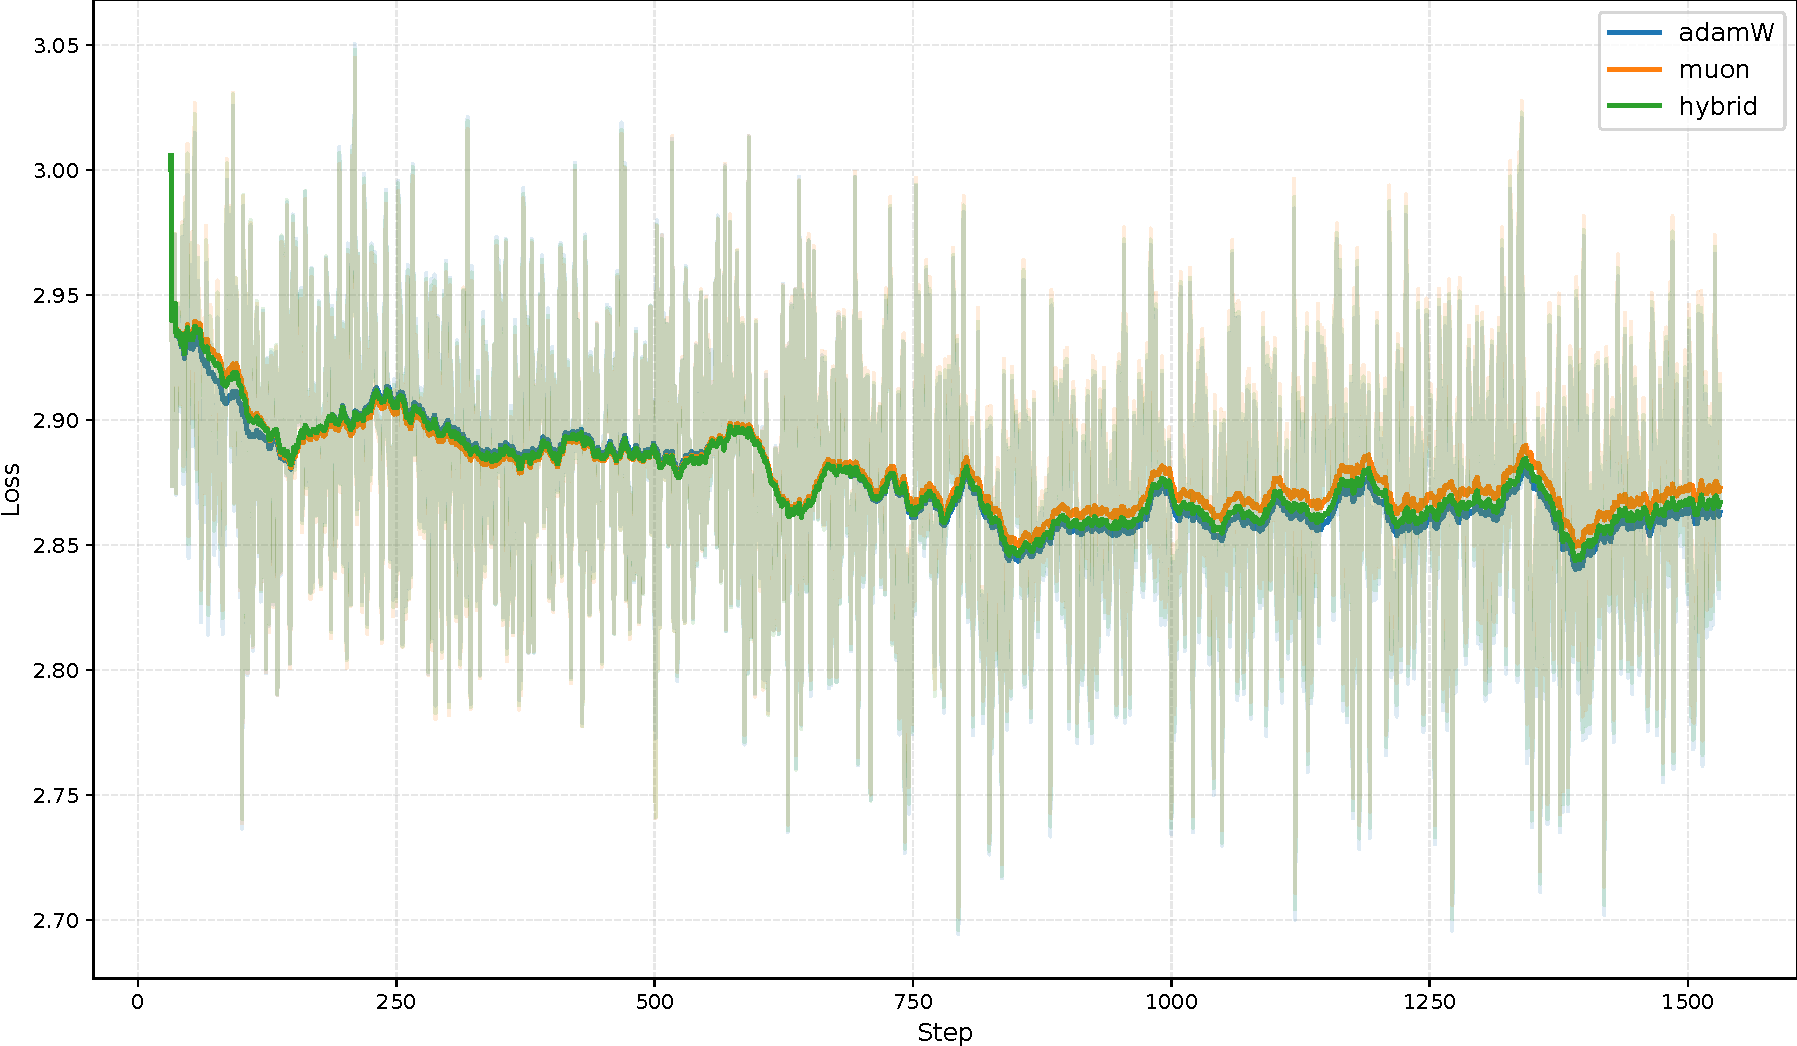
\includegraphics[width=0.7\linewidth]{train_loss_plot.pdf}
	\caption{Training loss versus optimization step for the three optimizer
		configurations. Each curve is smoothed with a moving-average window of
		50 steps}
	\label{fig:loss_curves}
\end{figure}

\section{Discussion}

Our results reveal that all three optimization strategies converge to comparable
performance on both training loss and downstream benchmarks, with differences in
average accuracy smaller than 0.3 percentage points. The Hybrid approach achieves
the highest average score (0.5260), marginally outperforming AdamW (0.5254)
and Muon (0.5230), yet these gaps fall well within the range of statistical
noise given that each configuration was trained only once. We attribute the overall
parity to two compounding factors. The Qwen2.5-0.5B model is sufficiently small
that AdamW already navigates its optimization landscape efficiently, leaving
little room for more sophisticated update rules to demonstrate an advantage.
Furthermore, the effective batch size of 64 produces noisy gradient estimates
that obscure the signal upon which Muon's orthogonal update relies; prior work
has shown that Muon's benefits become more pronounced at larger batch sizes.
Despite this, neither Muon nor the Hybrid method introduced training instability,
suggesting that both are safe drop-in replacements for AdamW under the resource
constraints.

\section{Limitations}
Several limitations constrain the conclusions that can be drawn from this study.


\paragraph{Single-server variance.}
Although all experiments targeted identical hardware,
they were executed on physically distinct servers.
Background system load, thermal throttling, and driver-level
non-determinism can all influence wall-clock timings. This is most evident in
the efficiency table, where the Hybrid optimizer reports a shorter training time
and higher token throughput than both simpler methods despite managing three
optimizer states - a result that is counterintuitive and likely reflects
favorable scheduling conditions rather than a genuine algorithmic advantage.
Efficiency conclusions should therefore be treated as indicative rather than
definitive, and ideally all runs should be repeated on a single, thermally
stable machine with controlled system load.

\paragraph{Single training run per configuration.}
Each optimizer was trained exactly once
with a fixed random seed. Without multiple independent runs, it is impossible to
estimate the variance of the reported metrics or to determine whether observed
differences in downstream accuracy are statistically meaningful. Best practice
would involve at least three to five runs per configuration with different seeds,
from which means and standard deviations can be reported. The current setup cannot
distinguish genuine optimizer effects from seed-specific artifacts.

\paragraph{No hyperparameter search.}
The hyperparameters for each optimizer - most
critically the learning rates - were set based on published recommendations
rather than tuned for this specific model, dataset, and training budget.
Muon in particular is sensitive to its learning rate and Newton–Schulz iteration
count, and a systematic sweep might reveal configurations where it outperforms
AdamW more clearly. As reported, the comparison is fair in the sense that all
optimizers use broadly reasonable settings, but it may inadvertently favor AdamW,
for which the chosen learning rate is well-established.

\paragraph{Limited training scale.}
At 1500 steps with an effective batch size of 64, the
total number of training tokens is modest (<100M tokens). Optimizer differences that manifest
over longer training horizons or at larger batch sizes may not be observable
within this budget. Scaling the experiment to larger models, longer schedules,
or higher batch sizes would be necessary to draw broader conclusions about the
relative merits of Muon-based strategies.

\paragraph{Benchmark sensitivity.}
Zero-shot evaluation on five benchmarks, each of which
has its own variance, compounds the difficulty of drawing firm conclusions
from single-run results. Task-level scores such as ARC-Challenge can fluctuate
by several tenths of a percent across evaluation runs depending on prompt
formatting and tokenization details.


\section{Conclusion}

We presented a systematic comparison of three optimization strategies for
continued pre-training of the Qwen2.5-0.5B language model: a standard AdamW
baseline, a Moonlight Muon configuration that applies orthogonal gradient updates
to internal 2D weight matrices, and a depth-stratified Hybrid approach that
restricts Muon to the first 12 transformer layers while using AdamW for deeper
layers and scalar parameters. Across five zero-shot reasoning benchmarks and 1500
training steps, all three methods converge at nearly identical rates and achieve
comparable downstream accuracy, with the Hybrid approach reaching the highest
aggregate score of 0.5260.

These findings suggest that Muon and Hybrid strategies are viable alternatives
to AdamW that introduce no instability, even under resource-constrained conditions
with small effective batch sizes. At the same time, they do not demonstrate a
clear practical advantage over the well-established AdamW baseline in this regime,
consistent with the hypothesis that Muon's orthogonalization benefits are most
pronounced at larger batch sizes and model scales.

\begin{thebibliography}{9}

	\bibitem{qwen}
	Qwen Team. Qwen2.5-0.5B.
	\url{https://huggingface.co/Qwen/Qwen2.5-0.5B}

	\bibitem{owt}
	Elriggs. openwebtext-100k. \url{https://huggingface.co/datasets/Elriggs/openwebtext-100k}

	\bibitem{lmharness}
	EleutherAI. Language Model Evaluation Harness.
	\url{https://github.com/EleutherAI/lm-evaluation-harness}

	\bibitem{muon}
	Moonshot AI. Moonlight / Muon optimizer.
	\url{https://github.com/MoonshotAI/Moonlight}

\end{thebibliography}

\end{document}
